\documentclass[11pt,a4paper]{article}
\usepackage[utf8]{inputenc}
\usepackage{amsmath}
\usepackage{amsfonts}
\usepackage{amssymb}
\usepackage{graphicx}
\usepackage{lmodern}
\usepackage{fourier}
\usepackage{enumitem}
\usepackage{amsthm} 
\usepackage{tikz}
\usepackage{tkz-euclide}
\usepackage{wrapfig}
\usepackage[romanian]{babel}
\usetikzlibrary{calc}
\newcommand\mytheta{110} %angle theta
\usetikzlibrary{angles,quotes,decorations.pathreplacing,patterns}
\usepackage[left=2cm,right=2cm,top=2cm,bottom=2cm]{geometry}
\author{Neacșu Andrei}
\title{Teorie și formule}
\date{}
\newlist{Properties}{enumerate}{2}
\setlist[Properties]{label=P \arabic*., font=\textbf, itemindent=*}
\newtheorem{theorem}{Teorema}
\newtheorem{corollary}{Corolar}[subsection]


\begin{document}
\maketitle
\section{Partea întreagă și partea fracționară a unui număr real}
 Fie $x\in \mathbb{R}$, atunci $\exists k \in \mathbb{Z}$ cu $k \leq x < k+1$. 

	$\bullet$ Se numește partea întreagă a numărului $x$ cel mai mare număr întreg, mai mic decât $x$.

$\bullet$	Prin definiție, partea fracționară a numărului real $x$ este $\{x\}=x-\lfloor x \rfloor$; evident $\{x\} \in [0,1)$.
\subsection{Proprietăți}
\begin{Properties}
  \item $x-1 < \lfloor x \rfloor \leq x,  \forall x \in \mathbb{R}$. 
  \item $x <k \Longleftrightarrow \lfloor x \rfloor < k, \forall x \in \mathbb{R}, k \in \mathbb{Z}$.
  \item $\lfloor k + \alpha \rfloor =k, \forall k \in \mathbb{Z}, \alpha \in [0,1)$.
  \item $\lfloor x + k \rfloor = \lfloor x \rfloor +k, \forall x \in \mathbb{R}, k \in \mathbb{Z}$.
  \item $\{x+k\}=\{x\}, \forall x \in \mathbb{R}, k \in \mathbb{Z}$.
  \item $\lfloor \lfloor x \rfloor \rfloor=\lfloor x \rfloor, \{\{x\}\}=\{x\}, \lfloor \{x\} \rfloor=0, \forall x \in \mathbb{R}$.
  \item Dacă $x, y \in \mathbb{R}$ și $\lfloor x \rfloor = \lfloor y \rfloor$, atunci $\lvert x-y \rvert <1$.
  \item $\{x\}=\{y\} \Longleftrightarrow (x-y)\in \mathbb{Z}, \forall x, y \in \mathbb{R}$.
  \item $\lfloor x \rfloor+ \lfloor y \rfloor \leq \lfloor x+y \rfloor \leq  \lfloor x \rfloor+ \lfloor y \rfloor +1; \forall x, y \in \mathbb{R}$.
  \item  $\lfloor -x \rfloor + \lfloor x \rfloor = -1, \forall x \in \mathbb{R} \setminus \mathbb{Z}$.
  \item $\lfloor x \rfloor + \left\lfloor x + \frac{1}{n} \right\rfloor + \left\lfloor x + \frac{2}{n} \right\rfloor + \ldots +  \left\lfloor x + \frac{n-1}{n} \right\rfloor = \lfloor nx \rfloor, \forall x \in \mathbb{R}, n \in \mathbb{N}^*$.
  \item Exponentul numărului natural prim $p$ din descompunerea în factori primi a numărului $n!$ este:\[ \left\lfloor \frac{n}{p}  \right\rfloor + \left\lfloor \frac{n}{p^2} \right\rfloor +\left\lfloor \frac{n}{p^3}\right\rfloor + \ldots \]
\end{Properties}

\section{Ecuația de gradul II}
Fie $a, b, c \in \mathbb{R}, a\neq 0$. Se numește ecuația de gradul II: $ax^2 +bx+c=0$.
\subsection{Rezolvarea ecuației de gradul II}
Soluțiile ecuației de gradul II se pot afla utilizând formula: $x_{1,2}= \frac{-b \pm \sqrt{b^2-4ac}}{2a}$
\subsection{Relațiile lui Viete}
$ \left\{
    \begin{aligned}
      & x_1 + x_2 = \frac{-b}{a}\\
      & x_1x_2=\frac{c}{a}
    \end{aligned}
  \right.$
  
  $$ax^2+bx+c=0 \Longleftrightarrow x^2 - (x_1+x_2)x +x_1x_2 = 0$$
  \section{Logaritmi}
  Fie $a>0, a \neq 1$ și $x>0$. Unicul număr real $y$ cu proprietatea $a^y=x$ se numește \textit{logaritmul} numărului $x$ în baza $a$ și se notează $\log_a x$.
  Astfel, $\log_a x = y \Leftrightarrow a^y = x$.
  \subsection{Observații}
  $\bullet$ Dacă $a = 10$, numărul $\log_{10} x = \lg x$ se numește logaritmul zecimal al lui $x$.\\
  $\bullet$ Dacă $a = e$, numărul $\log_e x = \ln x$ se numește logaritmul natural al lui $x$.
  \subsection{Proprietăți}
  \begin{Properties}
  \item $a^{\log_a x} = x, \forall x > 0$;
  \item $\log_a a^x = x, \forall x \in \mathbb{R}$;
  \item $\log_a a = 1, \forall a > 0, a \neq 1$;
  \item $\log_a 1 = 0, \forall a > 0, a \neq 1$;
  \item $x^{\log_a y}= y^{\log_a x}$;
  \item $\log_ax + \log_ay = \log_a(xy), \forall x, y > 0$;
  \item $\log_ax - \log_ay = \log_a(\frac{x}{y}), \forall x, y > 0$;
  \item $\log_ax^p = p \cdot \log_ax, \forall x > 0, \forall p \in \mathbb{R}$;
  \item $\log_{a^p}x = \frac{1}{p} \cdot \log_ax, \forall x > 0, \forall p \in \mathbb{R}^*$;
  \item $\log_ax = \frac{\log_bx}{\log_ba}, \forall a, b, x > 0; a, b \neq	 1$;
  \item $\log_ab \cdot \log_bc = \log_ac, \forall a, b, c > 0; a, b \neq 1$;
  \item $\log_ab = \frac{1}{\log_ba}, \forall a, b > 0; a, b \neq 1$.
  \end{Properties}
  Consecință: $\log_ax = \frac{\lg x }{\lg a} = \frac{\ln x }{\ln a}$
  \section{Numere Complexe}

Se definește mulțimea numerelor complexe ca: \quad
$\mathbb{C} = \mathbb{R} \times \mathbb{R} = \{ (x,y) \mid x,y \in \mathbb{R} \},
$\quad
înzestrată cu operațiile:

\begin{itemize}
    \item \textbf{Adunare:} \qquad $(x_1,y_1) + (x_2,y_2) = (x_1+x_2, y_1+y_2)$
    
    \item \textbf{Înmulțire:} \quad $
    (x_1,y_1) \cdot (x_2,y_2) = (x_1x_2 - y_1y_2, x_1y_2 + x_2y_1)$
\end{itemize}

Prin această corespondență, elementul \((x,y)\) se notează și ca:
$z = x + yi$ (forma algebrica), unde \(i\) este unitatea imaginară, cu proprietatea \(i^2 = -1\).
\subsection{Conjugatul unui număr complex}
Conjugatul unui număr complex \(z = x + yi\) se notează \(\overline{z}\) și se definește ca:
\[
\overline{z} = x - yi
\]

\textbf{Proprietăți:}  
\begin{Properties}
    \item \(\overline{\overline{z}} = z\)
    \item \(\overline{z + w} = \overline{z} + \overline{w}, \quad \forall w \in \mathbb{C}\)
    \item \(\overline{z \cdot w} = \overline{z} \cdot \overline{w}, \quad \forall w \in \mathbb{C}\)
    \item $\overline{z^n} = \left(\overline{z}\right)^n, \quad \forall n \in \mathbb{N}$
    \item $\arg\left(\overline{z}\right) = -\arg(z)$
    \item $\overline{\left(\frac{z}{w}\right)}=\frac{\overline{z}}{\overline{w}},\quad \forall w \in \mathbb{C}$
\end{Properties}
\subsection{Modulul unui număr complex}
Fie $z=x+yi$ un număr complex. Definim modulul numărului z: \quad $|z| = \sqrt{x^2 + y^2}$

\noindent\textbf{Proprietăți:}
\begin{Properties}
\item $|z| \in \mathbb{R}_+, |z|  \geq 0$; \quad Egalitate $\Leftrightarrow z=0$
\item $\left|z_1+z_2\right| \leq \left|z_1\right|+\left|z_2\right|, \quad \forall	z_1, z_2 \in \mathbb{C}$; \quad Egalitate $\Leftrightarrow \exists \lambda \in \mathbb{R}_+ , z_2 = \lambda \cdot z_1$
\item $\left|z_1 \cdot z_2\right| = \left|z_1\right| \cdot \left|z_2\right|, \quad \forall z_1, z_2 \in \mathbb{C}$
\item $\left|z^n\right| = |z|^n, \quad \forall n \in \mathbb{N}$
\item $\left|\frac{z_1}{z_2}\right| = \frac{\left|z_1\right|}{\left|z_2\right|}, \quad \forall z_1, z_2 \in \mathbb{C}$ 
 \item $z \cdot \overline{z} = |z|^2$
 \item $\left|\overline{z}\right| = |z|$
\end{Properties}
\subsection{Forma trigonometrică și exponențială}
Fie \(z = x + yi\) un număr complex. Definim:

 \textbf{Argumentul:} \qquad
$\arg(z)=\theta$ cu: \,$
\cos \theta = \frac{x}{|z|}, \quad \sin \theta = \frac{y}{|z|}$

 \textbf{Forma trigonometrică:} \qquad $
z = |z|(\cos\theta + i\sin\theta) $

\textbf{Forma exponențială:} \qquad $
z = |z| e^{i\theta}$
\begin{theorem}
Pentru orice \, $\theta \in [0, 2\pi)$, \, are loc identitatea:
$$e^{i\theta} = \cos\theta + i\sin\theta$$
\end{theorem}
\begin{theorem}[Moivre]
Pentru orice \, $\theta \in [0, 2\pi)$  și $n \in \mathbb{N}$ \, are loc relația:
 $$\left(\cos\theta+isin\theta\right)^n = \cos{n\theta}+i\sin{n\theta} $$
\end{theorem}
\begin{theorem}[Rădăcinile de ordin $n$ ale unui număr complex]
Fie $z \in \mathbb{C}$, $z \neq 0$, scris în forma trigonometrică
\[
z = |z|\cdot(\cos\theta+i\sin\theta), \quad \theta \in [0, 2\pi).
\]
Rădăcinile de ordin $n$ ale lui $z$ sunt numerele complexe
\[
\omega_k = \sqrt[n]{|z|}\cdot\, \left( \cos \left( \frac{\theta + 2k\pi}{n}\right)+i\sin\left(\frac{\theta + 2k\pi}{n}\right)\right), 
\quad k = \overline{0,1,2,\dots,n-1}.
\]
\end{theorem}

\subsection{Interpretare geometrică}
\begin{corollary}
Înmulțirea unui număr complex cu $e^{i\phi}=\cos\phi+i\sin\phi$ reprezintă o \textbf{rotație} în planul complex în sens trigonometric, cu unghiul $\phi$, în jurul originii.
\end{corollary}
\begin{corollary}
Înmulțirea succesivă cu $e^{i\phi}$ și $e^{i\psi}$ este echivalentă cu
înmulțirea cu $e^{i(\phi+\psi)}$, corespunzând compunerii rotațiilor.
\end{corollary}
\begin{corollary}
Rădăcinile de ordin $n$ ale unui număr complex nenul sunt puncte echidistante
pe cercul de rază $\sqrt[n]{|z|}$ și centru în origine, corespunzătoare
vârfurilor unui poligon regulat cu $n$ laturi.
\end{corollary}
\setcounter{theorem}{0}
  \section{Inegalități cunoscute}

\begin{theorem}[Inegalitatea mediilor]
Pentru $x_1, x_2, \dots, x_n > 0$, are loc lanțul de inegalități:
$$ \min(x_1, x_2, \dots, x_n) \leq \frac{n}{\sum_{i=1}^n \frac{1}{x_i}} \leq \sqrt[n]{\prod_{i=1}^n x_i} \leq \frac{1}{n} \sum_{i=1}^n x_i \leq \sqrt{\frac{1}{n} \sum_{i=1}^n x_i^2} \leq \max(x_1, x_2, \dots, x_n) $$
\end{theorem}
\begin{theorem}[Inegalitatea Cauchy-Schwarz]
Pentru orice $a_1, a_2, \dots, a_n, \, b_1, b_2,\dots b_n \in \mathbb{R}$ are loc:
$$ (a_1b_1 + a_2b_2 + ... + a_nb_n)^2 \leq (a_1^2 + a_2^2 + ... + a_n^2)(b_1^2 + b_2^2 + ... + b_n^2) $$
\end{theorem}
\begin{corollary}[Lema lui Titu] Pentru $b_1, b_2, \dots, b_n > 0$, are loc:\[\frac{a_1^2}{b_1} + \frac{a_2^2}{b_2} + \ldots + \frac{a_n^2}{b_n} \geq \frac{(a_1 + a_2 + \ldots + a_n)^2}{b_1 + b_2 + \ldots + b_n}\]
\end{corollary}
\begin{theorem}
Pentru $a,b,c \in \mathbb{R}$ are loc:
$$a^2+b^2+c^2 \ge ab+ac+bc \Leftrightarrow (a-b)^2+(a-c)^2+(b-c)^2 \ge 0$$
\end{theorem}
\section{Vectori}
Se numește vector $\overrightarrow{AB}$ mulțimea tuturor segmentelor orientate $\overline{CD}$ echipolente cu $\overline{AB}$. \[\overrightarrow{AB}=\{\overline{CD} \vert \overline{CD} \sim \overline{AB}\}\]
\subsection{Proprietăți ale înmulțirii cu scalari}
\begin{Properties}
\item $\alpha(\overrightarrow{AB}+\overrightarrow{CD})= \alpha\overrightarrow{AB}+\alpha\overrightarrow{CD}, \forall \alpha \in \mathbb{R}, \overrightarrow{AB}, \overrightarrow{CD}$ vectori.
\item $(\alpha + \beta)\overrightarrow{AB} = \alpha \overrightarrow{AB}+\beta \overrightarrow{AB}, \forall \alpha, \beta \in \mathbb{R}, \overrightarrow{AB}$ vector.
\item $(-1)\overrightarrow{AB}=\overrightarrow{BA}$.
\item $0 \cdot \overrightarrow{AB}=\overrightarrow{0}$.
\item $\alpha \cdot \overrightarrow{0} = \overrightarrow{0}, \forall \alpha \in \mathbb{R}$.
\end{Properties}
\subsection{Coliniaritate și paralelism}
Doi vectori $\overrightarrow{u}$ și $\overrightarrow{v}$ sunt coliniari $\Leftrightarrow \exists \lambda \in \mathbb{R}$ cu $\overrightarrow{u}= \lambda \cdot \overrightarrow{v}$.


Fie $\overline{AB}$ un segment orientat și $M \in AB $. $\frac{\overline{MA}}{\overline{MB}}=k$.
Pentru orice punct O din plan are loc relația: \[\overrightarrow{OM}=\frac{1}{1-k}\overrightarrow{OA}+\frac{-k}{1-k}\overrightarrow{OB}\]
\subsection{Centrul de greutate}
Fie $\triangle{ABC}$. Medianele $AP, BN$  și $ CM$ sunt concurente într-un punct notat $G$ = centrul de greutate al $\triangle{ABC}$.

Pentru orice punct $O \in \mathcal{P}$ are loc relația(Leibniz): \[\overrightarrow{OA}+\overrightarrow{OB}+\overrightarrow{OC}=3\overrightarrow{OG}\]
\subsection{Teorema bisectoarei}
Fie $\triangle{ABC}$ cu notațiile: $BC=a$, $AC=b$, $AB=c$. Bisectoarele $AA'$, $BB'$ și $CC'$ sunt concurente într-un punct notat $I$. Pentru orice punct $M \in \mathcal{P}$ are loc relația: \[\overrightarrow{MI}=\frac{1}{a+b+c}\left(a \cdot \overrightarrow{MA}+ b \cdot \overrightarrow{MB}+ c \cdot \overrightarrow{MC}\right)\]
\subsection{Teorema lui Menelaus}
Fie $\triangle{ABC}$ și punctele $M \in AB$, $P \in BC$, $N \in AC$. Acestea sunt coliniare dacă și numai dacă: \[\frac{AM}{MB}\cdot \frac{BP}{PC} \cdot \frac{CN}{NA}=1\]
\subsection{Teorema lui Ceva}
Fie $\triangle{ABC}$ și punctele $M \in AB$, $N \in BC$, $P \in AC$. Dreptele $AN, CM, BP$\, sunt concurente dacă și numai dacă: \[\frac{AM}{MB}\cdot \frac{BN}{NC} \cdot \frac{CP}{PA}=1\]
\subsection{Teorema Van Aubel}
Fie $\triangle{ABC}$ și cevienele $AN \cap CM \cap BP =\{T\}$. Are loc relația: \[\frac{AT}{TN}=\frac{AM}{MB}+\frac{AP}{PC}\]
\subsection{Produsul scalar}
Fie $\overrightarrow{u}$ și $\overrightarrow{v}$ vectori. Se numește produs scalar numărul real: \[\langle\overrightarrow{u},\overrightarrow{v}\rangle = \overrightarrow{u} \cdot \overrightarrow{v} = \left \Vert \overrightarrow{u} \right \Vert \cdot \left \Vert \overrightarrow{v} \right \Vert \cdot \cos(\widehat{\overrightarrow{u},\overrightarrow{v}}) \]
$$\overrightarrow{u} \perp \overrightarrow{v} \Leftrightarrow \langle\overrightarrow{u},\overrightarrow{v}\rangle  \hspace{3pt} =   0. $$
\begin{Properties}
\item $\overrightarrow{u} \perp \overrightarrow{v} \Leftrightarrow \langle\overrightarrow{u},\overrightarrow{v}\rangle  \hspace{3pt} =   0, \forall \overrightarrow{u},\overrightarrow{v}$ vectori.
\item $\overrightarrow{u}\cdot(\overrightarrow{v}+\overrightarrow{w}) = \overrightarrow{u} \cdot \overrightarrow{v} + \overrightarrow{u} \cdot \overrightarrow{w}, \forall \overrightarrow{u}, \overrightarrow{v}, \overrightarrow{w} $ vectori.
\item $\overrightarrow{u} \cdot \overrightarrow{u} = \left \Vert \overrightarrow{u} \right \Vert ^2, \forall \overrightarrow{u}$ vector.
\item $\langle\alpha \overrightarrow{u}, \beta\overrightarrow{v}\rangle = \alpha\beta \langle\overrightarrow{u}, \overrightarrow{v}\rangle, \forall \alpha,\beta \in \mathbb{R}, \overrightarrow{u}, \overrightarrow{v}$ vectori.
\item $\hat{i} \cdot \hat{i} = 1 \quad \hat{j} \cdot \hat{j} = 1 \quad \hat{k} \cdot \hat{k} = 1 \quad \hat{i} \cdot \hat{j} = \hat{i}\cdot\hat{k}=\hat{j}\cdot\hat{i}=\hat{j}\cdot\hat{k}=\hat{k}\cdot\hat{i}=\hat{k}\cdot\hat{j}=0$.
\item $\langle\overrightarrow{0}, \overrightarrow{u}\rangle = 0, \forall \overrightarrow{u}$ vector.
\end{Properties}
\section{Trigonometrie}
\begin{wrapfigure}[8]{l}{0.3\textwidth}
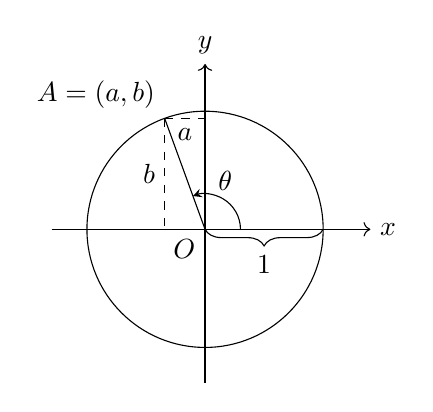
\begin{tikzpicture}[scale=1.5]
\draw[->] (-1.3,0)--(1.4,0) node[right] {$x$};
\draw[->] (0,-1.3)--(0,1.4) node[above] {$y$};
\coordinate (O) at (0,0);
\coordinate[label=above left:${A = (a, b)}$] (A) at (\mytheta:1);
\coordinate (C) at (-0.34202,0);
\coordinate (S) at (0,0.939693);
\draw[dashed] (A)--(C);
\draw[dashed] (A)--(S);
\coordinate (E) at (1,0);
\node[below left] at (O) {$O$};
\draw (O) circle (1);
\draw (A) -- (O);
\draw[-stealth] ($(O)!0.3!(E)$) arc (0:\mytheta:0.3) node[midway, above] {$\theta$};
\draw[decorate, decoration={brace, mirror, amplitude=6pt}]
(O) -- (E) node[midway, below=6pt] {$1$};
\node[left] at (-0.34202,0.469846) {$b$};
\node[below] at (-0.17101,0.939693) {$a$};
\end{tikzpicture}
\caption{Cercul unitate}
\label{trig}
\end{wrapfigure}
Fie $\theta$ un unghi (figura \ref{trig}).
Definim următoarele funcții:
\begin{align*}
\sin(\theta) &= b, & \csc(\theta) &= \frac{1}{b},\\
\cos(\theta) &= a, & \sec(\theta) &= \frac{1}{a},\\
\tan(\theta) &= \frac{b}{a}, & \cot(\theta) &= \frac{a}{b}
\end{align*}

\noindent Domeniile de valori ale funcțiilor sunt:
\begin{align*}
\sin(\theta),\ \cos(\theta) &\in [-1, 1],\\
\tan(\theta),\ \cot(\theta) &\in (-\infty, \infty) \quad \text{(cu excepția discontinuităților)},\\
\sec(\theta),\ \csc(\theta) &\in (-\infty, -1] \cup [1, \infty).
\end{align*}

\subsection{Formule și identități}
\subsubsection{Identități pentru tangentă și contangentă} 
$$\tan(\theta)=\frac{\sin(\theta)}{\cos(\theta)} \quad\quad cot(\theta)=\frac{\cos(\theta)}{\sin(\theta)}$$
\subsubsection{Identități reciproce}
\begin{align*}
\sin(\theta) &= \frac{1}{\csc(\theta)} \quad\quad \csc(\theta) = \frac{1}{\sin(\theta)} \\
\cos(\theta) &= \frac{1}{\sec(\theta)} \quad\quad \sec(\theta) = \frac{1}{\cos(\theta)} \\
\tan(\theta) &= \frac{1}{\cot(\theta)} \quad\quad \cot(\theta) = \frac{1}{\tan(\theta)} \\
\end{align*}
\subsubsection{Identități Pitagoreice}
\begin{align*}
\sin^2(\theta) + \cos^2(\theta) &= 1 \\
1 + \tan^2(\theta) &= \sec^2(\theta) \\
1 + \cot^2(\theta) &= \csc^2(\theta)
\end{align*}
\subsubsection{Formule pentru unghi dublu}
\begin{align*}
\sin(2\theta) &= 2\sin(\theta)\cos(\theta) \\
\cos(2\theta) &= \cos^2(\theta) - \sin^2(\theta) \\
              &= 2\cos^2(\theta) - 1 \\
              &= 1 - 2\sin^2(\theta) \\
\tan(2\theta) &= \frac{2\tan(\theta)}{1 - \tan^2(\theta)}
\end{align*}
\subsubsection{Formule pentru jumătate de unghi}

\begin{align*}
\sin\left(\frac{\theta}{2}\right) &= \pm\sqrt{\frac{1 - \cos(\theta)}{2}} \\
\cos\left(\frac{\theta}{2}\right) &= \pm\sqrt{\frac{1 + \cos(\theta)}{2}} \\
\tan\left(\frac{\theta}{2}\right) &= \pm\sqrt{\frac{1 - \cos(\theta)}{1 + \cos(\theta)}} \\
\end{align*}
\subsubsection{Formule pentru suma și diferența unghiurilor}

\begin{align*}
\sin(\alpha \pm \beta) &= \sin(\alpha)\cos(\beta) \pm \cos(\alpha)\sin(\beta) \\
\cos(\alpha \pm \beta) &= \cos(\alpha)\cos(\beta) \mp \sin(\alpha)\sin(\beta) \\
\tan(\alpha \pm \beta) &= \frac{\tan(\alpha) \pm \tan(\beta)}{1 \mp \tan(\alpha)\tan(\beta)}
\end{align*}

\subsubsection{Formule de transformare din produs în sumă}

\begin{align*}
\sin(\alpha)\sin(\beta) &= \frac{1}{2} \left[ \cos(\alpha - \beta) - \cos(\alpha + \beta) \right] \\
\cos(\alpha)\cos(\beta) &= \frac{1}{2} \left[ \cos(\alpha - \beta) + \cos(\alpha + \beta) \right] \\
\sin(\alpha)\cos(\beta) &= \frac{1}{2} \left[ \sin(\alpha + \beta) + \sin(\alpha - \beta) \right] \\
\cos(\alpha)\sin(\beta) &= \frac{1}{2} \left[ \sin(\alpha + \beta) - \sin(\alpha - \beta) \right]
\end{align*}

\subsubsection{Formule de transformare din sumă în produs}

\begin{align*}
\sin(\alpha) + \sin(\beta) &= 2 \sin\left( \frac{\alpha + \beta}{2} \right) \cos\left( \frac{\alpha - \beta}{2} \right) \\
\sin(\alpha) - \sin(\beta) &= 2 \cos\left( \frac{\alpha + \beta}{2} \right) \sin\left( \frac{\alpha - \beta}{2} \right) \\
\cos(\alpha) + \cos(\beta) &= 2 \cos\left( \frac{\alpha + \beta}{2} \right) \cos\left( \frac{\alpha - \beta}{2} \right) \\
\cos(\alpha) - \cos(\beta) &= -2 \sin\left( \frac{\alpha + \beta}{2} \right) \sin\left( \frac{\alpha - \beta}{2} \right)
\end{align*}
\subsubsection{Formule de complementaritate}

\begin{align*}
\sin\left( \frac{\pi}{2} - \theta \right) &= \cos(\theta) &\quad
\cos\left( \frac{\pi}{2} - \theta \right) &= \sin(\theta) \\
\csc\left( \frac{\pi}{2} - \theta \right) &= \sec(\theta) &\quad
\sec\left( \frac{\pi}{2} - \theta \right) &= \csc(\theta) \\
\tan\left( \frac{\pi}{2} - \theta \right) &= \cot(\theta) &\quad
\cot\left( \frac{\pi}{2} - \theta \right) &= \tan(\theta)
\end{align*}
\subsection{Teorema sinusurilor}
Fie $\triangle{ABC}$ cu notațiile: $BC=a$, $AC=b$, $AB=c$, $\widehat{BAC}=\widehat{A}, \widehat{ABC}=\widehat{B}, \widehat{ACB}=\widehat{C}, R= $ raza cercului circumscris.

$$\frac{a}{\sin A} = \frac{b}{\sin B} = \frac{c}{\sin C} = 2R$$
\subsection{Teorema cosinusurilor}

\begin{align*}
c^2 &= a^2 + b^2 - 2ab\cos\widehat{C} \\
b^2 &= a^2 + c^2 - 2ac\cos\widehat{B} \\
a^2 &= b^2 + c^2 - 2bc\cos\widehat{A}
\end{align*}
\subsection{Teorema tangentei}

\begin{align*}
\frac{a - b}{a + b} &= \frac{\tan\left( \frac{\widehat{A} - \widehat{B}}{2} \right)}{\tan\left( \frac{\widehat{A} + \widehat{B}}{2} \right)} \\
\frac{b - c}{b + c} &= \frac{\tan\left( \frac{\widehat{B} - \widehat{C}}{2} \right)}{\tan\left( \frac{\widehat{B} + \widehat{C}}{2} \right)} \\
\frac{c - a}{c + a} &= \frac{\tan\left( \frac{\widehat{C} - \widehat{A}}{2} \right)}{\tan\left( \frac{\widehat{C} + \widehat{A}}{2} \right)}
\end{align*}

\subsection{Formula Mollweide}

\begin{align*}
\frac{a - b}{c} &= \frac{\sin\left( \frac{\widehat{A} - \widehat{B}}{2} \right)}{\cos\left( \frac{\widehat{C}}{2} \right)} \\
\frac{a + b}{c} &= \frac{\cos\left( \frac{\widehat{A} - \widehat{B}}{2} \right)}{\sin\left( \frac{\widehat{C}}{2} \right)}
\end{align*}
\setcounter{theorem}{0}
\section{Aplicații ale trigonometriei în geometrie}
\subsection{Aria unui triunghi scalen}
Fie $\triangle ABC$ cu notațiile: $BC=a$, $AC=b$, $AB=c$; $AA_1 \perp BC, A_1 \in BC$, $BB_1 \perp AC, B_1 \in AC$, $CC_1 \perp AB, C_1 \in AB$.
\begin{align*}
S_{ABC} &= \frac{a \cdot AA_1}{2} = \frac{b \cdot BB_1}{2} = \frac{c \cdot CC_1}{2}\\
 S_{ABC} &= \frac{a \cdot c \cdot \sin{\widehat{B}}}{2} = \frac{a \cdot b \cdot \sin{\widehat{C}} }{2} = \frac{b \cdot c \cdot \sin{\widehat{A}}}{2} \\
 S_{ABC} &= \sqrt{p(p-a)(p-b)(p-c)}, p = \frac{a+b+c}{2}\\
 S_{ABC} &= \frac{a  b  c}{4R} \Leftrightarrow 4RS_{ABC} = abc
\end{align*}
\subsection{Relații metrice în triunghiul oarecare}
 \begin{wrapfigure}{R}{0.3\textwidth}
 \centering
 \vspace{-55pt}
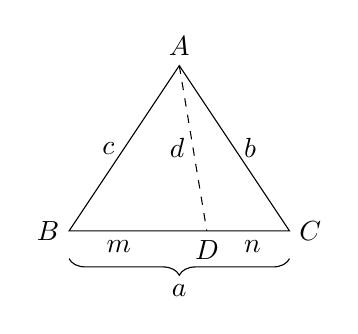
\begin{tikzpicture}[scale=0.7]
\coordinate (A) at (0,3);
\coordinate (B) at (-2,0);
\coordinate (C) at (2,0);
\coordinate (D) at (0.5,0);
\draw (A)--(B)--(C)--cycle;
\draw[dashed] (A)--(D);
\node[above] at (A) {$A$};
\node[left] at (B) {$B$};
\node[right] at (C) {$C$};
\node[below] at (D) {$D$};
\node[left] at (-1,1.5) {$c$};
\node[right] at (1,1.5) {$b$};
\node[below left] at (-0.7,0) {$m$};
\node[below right] at (1,0) {$n$};
\node[right] at (-0.35,1.5){$d$};
\draw[decorate, decoration={brace, mirror, amplitude=6pt, raise=10pt}]
(B) -- (C) node[midway, below=16pt] {$a$};
\end{tikzpicture}
\caption{Teorema lui Stewart}
\label{th_stew}
\vspace{1em}
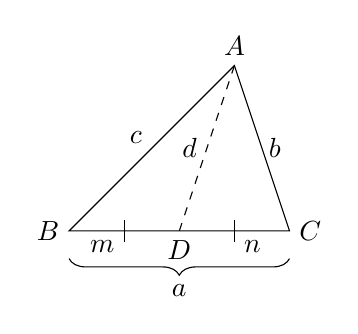
\begin{tikzpicture}[scale=0.7]
\coordinate (A) at (1,3);
\coordinate (B) at (-2,0);
\coordinate (C) at (2,0);
\coordinate (D) at (0,0);
\draw (A)--(B)--(C)--cycle;
\draw[dashed] (A)--(D);
\node[above] at (A) {$A$};
\node[left] at (B) {$B$};
\node[right] at (C) {$C$};
\node[below] at (D) {$D$};
\node[left] at (-.5,1.7) {$c$};
\node[right] at (1.45,1.5) {$b$};
\node[below left] at (-1,0) {$m$};
\node[below right] at (1,0) {$n$};
\node[right] at (-0.12,1.5){$d$};
\draw[decorate, decoration={brace, mirror, amplitude=6pt, raise=10pt}]
(B) -- (C) node[midway, below=16pt] {$a$};
\tkzMarkSegment[pos=.5,mark=|](B,D)
\tkzMarkSegment[pos=.5,mark=|](D,C)
\end{tikzpicture}
\caption{Teorema medianei}
\label{th_med}
\end{wrapfigure}
\begin{theorem}[Stewart]
Fie $\triangle{ABC}$ cu notațiile: $BC=a$, $AC=b$, $AB=c$. Fie ceviana $AD, D \in [BC]$. Notăm: $BD=m$, $DC=n$, $AD=d$(Vezi figura  \ref{th_stew}). Are loc relația: \[a(mn+d^2)=b^2m+c^2n\]
\end{theorem}
\noindent \textbf{Mnemonică:} Pentru a reține mai ușor formula, se poate folosi expresia în limba engleză: \textit{„A \textbf{man} and his \textbf{dad} put a \textbf{bomb} in the \textbf{sink}”}.
\vspace{1em}

\begin{corollary}[Mediana]
O consecință directă a Teoremei lui Stewart este Teorema medianei \,(cazul particular\,$m=n=\frac{1}{2} a$,\, figura \ref{th_med}): \[d=\frac{\sqrt{2(b^2+c^2)-a^2}}{2}\]
\end{corollary}
\vspace{1em}
\noindent \textbf{Observație:} În triunghiuri isoscele mediana AD este perpendiculară pe latura BC și teorema devine identică cu cea a lui Pitagora.
\end{document}
